\documentclass[14pt]{extarticle}

\usepackage{amsmath}
\usepackage{amsfonts}
\usepackage{graphicx}
\usepackage{nicefrac}
\usepackage{subfigure}
\usepackage{algorithm}
\usepackage{paralist}
\usepackage[geometry]{ifsym}
\usepackage{rotating}
\usepackage[framed,numbered,autolinebreaks,useliterate]{mcode}
\usepackage[normalem]{ulem}
\usepackage{varwidth}
% \usepackage{cite}
% \usepackage{color}
\usepackage{algpseudocode}
% \bibliographystyle{amsplain}

\addtolength{\oddsidemargin}{-.2in}
    \addtolength{\evensidemargin}{-.5in}
    \addtolength{\textwidth}{0.5in}

    \addtolength{\topmargin}{-.5in}
    \addtolength{\textheight}{0.35in}

\sloppy                 % makes TeX less fussy about line breaking

\pagestyle{plain}           % use just a plain page number

\numberwithin{equation}{section}    % add the section number to the equation label

\usepackage{fancyheadings}

\newcommand{\com}[1]{\texttt{#1}}
\newcommand{\DIV}{\ensuremath{\mathop{\mathbf{DIV}}}}
\newcommand{\GRAD}{\ensuremath{\mathop{\mathbf{GRAD}}}}
\newcommand{\CURL}{\ensuremath{\mathop{\mathbf{CURL}}}}
\newcommand{\CURLt}{\ensuremath{\mathop{\overline{\mathbf{CURL}}}}}
\newcommand{\nullspace}{\ensuremath{\mathop{\mathrm{null}}}}


\newcommand{\FrameboxA}[2][]{#2}
\newcommand{\Framebox}[1][]{\FrameboxA}
\newcommand{\Fbox}[1]{#1}

%\usepackage[round]{natbib}

\newcommand{\half}{\mbox{\small \(\frac{1}{2}\)}}
\newcommand{\hf}{{\frac 12}}
\newcommand {\HH}  { {\bf H} }
\newcommand{\hH}{\widehat{H}}
\newcommand{\hL}{\widehat{L}}
\newcommand{\bmath}[1]{\mbox{\bf #1}}
\newcommand{\hhat}[1]{\stackrel{\scriptstyle \wedge}{#1}}
\newcommand{\R}{{\rm I\!R}}
\newcommand {\D} {{\vec{D}}}
\newcommand {\sg}{{\hsigma}}
%\renewcommand{\vec}[1]{\ensuremath{\mathbf{#1}}}
\newcommand{\E}{\vec{E}}
\renewcommand{\H}{\vec{H}}
\newcommand{\J}{\vec{J}}
\newcommand{\dd}{d^{\rm obs}}
% \newcommand{\F}{\vec{F}}
\newcommand{\C}{\vec{C}}
\newcommand{\s}{\vec{s}}
\newcommand{\N}{\vec{N}}
\newcommand{\M}{\vec{M}}
\newcommand{\A}{\vec{A}}
\newcommand{\B}{\vec{B}}
\newcommand{\w}{\vec{w}}
\newcommand{\nn}{\vec{n}}
\newcommand{\cA}{{\cal A}}
\newcommand{\cQ}{{\cal Q}}
\newcommand{\cR}{{\cal R}}
\newcommand{\cG}{{\cal G}}
\newcommand{\cW}{{\cal W}}
\newcommand{\hsig}{\hat \sigma}
\newcommand{\hJ}{\hat \J}
\newcommand{\hbeta}{\widehat \beta}
\newcommand{\lam}{\lambda}
\newcommand{\dt}{\delta t}
\newcommand{\kp}{\kappa}
\newcommand {\lag} { {\cal L}}
\newcommand{\zero}{\vec{0}}
\newcommand{\Hr}{H_{red}}
\newcommand{\Mr}{M_{red}}
\newcommand{\mr}{m_{ref}}
\newcommand{\thet}{\ensuremath{\mbox{\boldmath $\theta$}}}
\newcommand{\curl}{\ensuremath{\nabla_{\wedge}\,}}
\renewcommand{\div}{\nabla\cdot\,}
\newcommand{\grad}{\ensuremath{\nabla}}
\newcommand{\dm}{\delta m}
\newcommand{\gradh}{\ensuremath{\nabla}_h}
\newcommand{\divh}{\nabla_h\cdot\,}
\newcommand{\curlh}{\ensuremath{\nabla_h\times\,}}
\newcommand{\curlht}{\ensuremath{\nabla_h^T\times\,}}
\newcommand{\Q}{\vec{Q}}
\renewcommand{\J}{\vec J}
\renewcommand{\J}{\vec J}
\renewcommand{\u}{\vec u}
\newcommand{\f}{\vec f}
\newcommand{\n}{\vec n}
\renewcommand{\v}{\vec v}
\newcommand{\phiv}{\vec \phi}
% \usepackage[authoryear,numbers,square,sort,comma,colon,]{natbib}
% \usepackage[numbers/]{natbib}
% \usepackage[square,sort,comma,numbers]{natbib}
\renewcommand{\ne}{N\'ed\'elec elements }


\newcommand{\me}{Maxwell's equations }

\newcommand{\partialt}[1]{\frac{\partial #1}{\partial t}}
\newcommand{\cref}[1]{(\ref{#1})}
% \newcommand{\Ct}{\ensuremath{C^{\mbox{\tiny{T}}}}
\newcommand{\Ct}{\ensuremath{C^{\mbox{\tiny{T}}}}}
% \renewcommand{\baselinestretch}{1.40}\normalsize
\usepackage{setspace}
\usepackage{amsthm}
\newtheorem{prop}{Proposition}[section]
\DeclareMathAlphabet{\mathpzc}{OT1}{pzc}{m}{it}

\DeclareFontFamily{OT1}{pzc}{}
\DeclareFontShape{OT1}{pzc}{m}{it}{<-> s * [0.900] pzcmi7t}{}
\DeclareMathAlphabet{\mathpzc}{OT1}{pzc}{m}{it}

\onehalfspacing
\begin{document}
\pagestyle{fancyplain}
\fancyhead{}
\fancyfoot{} % clear all footer fields
\fancyfoot[LE,RO]{\thepage \hspace{-5mm}}
\fancyfoot[LO,CE]{ \footnotesize{ Michael Wathen 7830121}}
\fancyfoot[CO,RE]{}
\pagecolor{cyan}

\title{Notes curl-curl vector-valued equation}
\author{Michael Wathen}
\maketitle

\section{Model}

Consider the vector-valued equation on the domain $\Omega \in \mathbb{R}^d$ where $d$ is the dimension of the problem (here we use $d = 2,3$):
\begin{equation} \label{system}
    \curl \curl \u + c(x,y) \u = \f, \ \ \mbox{in} \ \ \Omega
\end{equation}
with $\f \in L^2 (\Omega)^d$ as the right hand side. We will be considering Dirichlet boundary conditions:
\begin{equation} \label{bc}
    \u_\wedge \hspace{-.2mm} \n = g,
\end{equation}
on the boundary $\partial \Omega$.

This type of system arises in the Maxwell system. In fact, this is the form of the Schur complement of 1st order form of Maxwell's equations.

\section{Weak from}

To be able to discretise (\ref{system}) using the the finite element method (FEM) we first need to look at the weak form of the equations. We do this by multiplying through by a test function $\v$ and then integrating over the domain. This gives:
$$  \int_\Omega \curl \curl \u \cdot \v + c(x,y) \u \cdot \v\, dx = \int_\Omega \f \cdot \v \, dx, $$
together with integration by parts and Green's Formulas we arrive at the following equation
\begin{equation} \label{weakform}
    \int_\Omega \curl \u \ \curl \v + c(x,y) \u \cdot \v\, dx = \int_\Omega \f \cdot \v \, dx.
\end{equation}

We define the Stiffness matrix ($\mathcal{K}$) to be  $\int_\Omega \curl \u \ \curl \v \, dx$, the Mass matrix ($\mathcal{M}$) to be $ \int_\Omega c(x,y)\u \cdot \v \, dx$ and the right hand side vector ($\mathpzc{f}$) as $\int_\Omega \f \cdot \v \, dx$ to form the linear equation
\begin{equation} \label{eq:MatrixSystem}
    (\mathcal{K}+\mathcal{M}) u = \mathpzc{f}.
\end{equation}

\section{\ne}

\ne  of the first type \cite{Nedelec1980} are $H$(curl;$\Omega$)-conforming vector-valued finite elements that can be used to discretise the weak form of the curl-curl system given in (\ref{weakform}).



\subsection{\ne  of the first kind }

Before diving into the full finite element discretisation we need to derive the linear edge basis function. Here we will go through how one would derive both the basis functions on both tetrahedral and quadrilateral elements.

\subsubsection{Tetrahedral elements}




\begin{figure}[h!]
\centering
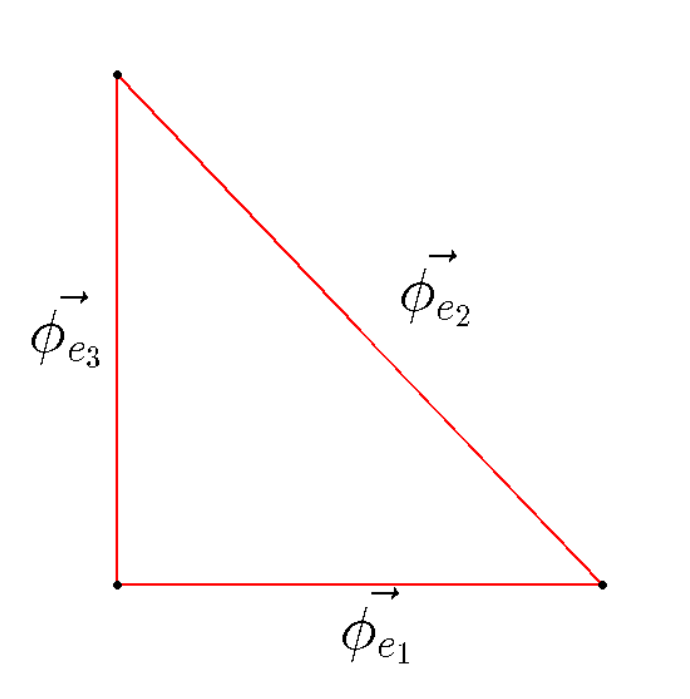
\includegraphics[width=6cm]{GridFigure/basisFuncsTets}
\caption{Tetrahedral reference cell}
\label{fig:tetBasis}
\end{figure}

\begin{equation}\label{eq:BasisFuncsTets}
    \phiv_{e_1} = \begin{pmatrix}
        1-\hat y\\ \hat x
    \end{pmatrix}, \  \phiv_{e_2} = \begin{pmatrix}
        -\hat y \\ \hat x
    \end{pmatrix}, \ \phiv_{e_3} = \begin{pmatrix}
        -\hat y\\ \hat x-1
    \end{pmatrix},
\end{equation}

\subsubsection{Quadrilateral elements}


\begin{figure}[h!]
\centering
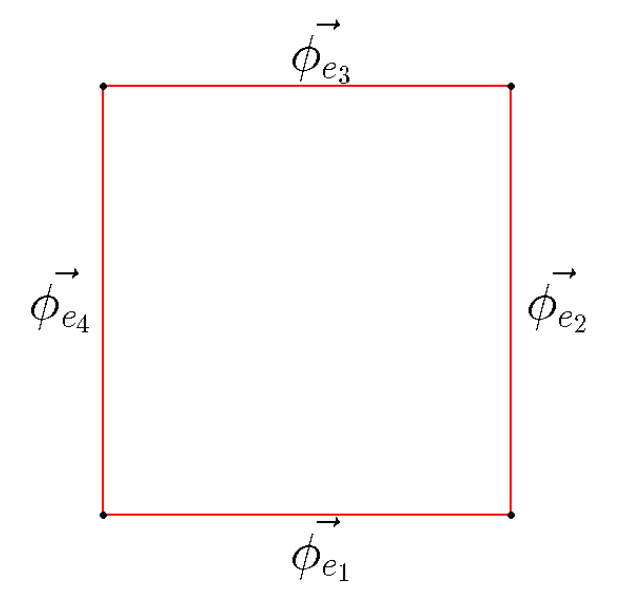
\includegraphics[width=6cm]{GridFigure/basisFuncsQuads}
\caption{Quadrilateral reference cell}
\label{fig:quadBasis}
\end{figure}

\begin{equation}\label{eq:BasisFuncsQuads}
    \phiv_{e_1} = \begin{pmatrix}
        1-\hat y\\0
    \end{pmatrix}, \  \phiv_{e_2} = \begin{pmatrix}
        0\\ \hat x
    \end{pmatrix}, \ \phiv_{e_3} = \begin{pmatrix}
        -\hat y\\0
    \end{pmatrix}, \  \phiv_{e_4} = \begin{pmatrix}
        0\\ \hat x-1
    \end{pmatrix}.
\end{equation}

% \subsection{Error}

\subsection{FEM grid construction}

In this subsection we will go over a way to form a uniform quad mesh to  be used in the FEM discretisation. Here I will denote $a(=0)$ and $b(=1)$ to be the  boundary of the domain and $n$ as the number of grid points. This means that for a uniform grid we will have $(n-1)^d$ cells (recall that $d$ is the dimension of the domain). From here we will be looking at the 2-dimensional problem, hence $d=2$.

The first things to decide is how to number the cells and edges of the grid. The way this ordering will effect the sparsity pattern of the matrix system given by (\ref{eq:MatrixSystem}) which could cause more fill when using direct methods but do not matter so much when using iterative methods. An example of an ordering one can use is given in figure~\ref{fig:grid}.
\begin{figure}[h!]
\centering
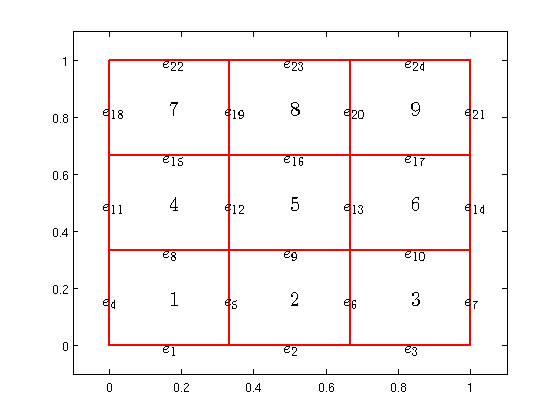
\includegraphics[width=10cm]{GridFigure/3x3Grid}
\caption{Example Grid}
\label{fig:grid}
\end{figure}

Using the ordering from figure~\ref{fig:grid}, one can then store what edge is defined in what cell as a matrix (see (\ref{eq:nnode})). Here we have recorded the edge elements in an anticlockwise orientation for each of the cells (the numbers in bold above each column of the matrix NNode).
\begin{equation} \label{eq:nnode}
\mbox{NNode}^T = \bordermatrix{
 ~&\bf{1}  &  \bf{ 2} &    \bf{3} &   \bf{4}  &   \bf{5} &   \bf{6} &   \bf{7} &   \bf{8} &   \bf{9}\cr
 ~&1  &   2 &    3 &    8  &   9 &   10 &   15 &   16 &   17\cr
    ~& 5   &  6 &    7    &12&    13    &14&    19    &20&    21\cr
    ~& 8   &  9   & 10 &   15 &   16 &   17 &   22 &   23 &   24\cr
     ~&4  &   5     &6&    11    &12&    13    &18&    19    &20\cr
}
\end{equation}



\subsection{Matrix assemble}


Take $c(x,y) = 1$ then the weak form of the problem is
$$ \int_\Omega \curl \u \ \curl \v + \u \cdot \v\, dx = \int_\Omega \f \cdot \v \, dx.$$
Defining
\begin{equation} \label{eq:discreteDef}
u = \sum_{i=1}^n u_i \phiv_a \ \ \mbox{and} \ \ \v = \sum_{j=1}^n v_j \phiv_j
\end{equation}
where $\phiv_{k}$ (where $k = a$ or $b$) are the basis functions defined in (\ref{eq:BasisFuncsQuads}) on the reference cell $(\hat x,\hat y)$. Substitute (\ref{eq:discreteDef}) into (\ref{weakform}) gives
\begin{equation} \label{eq:discreteWF}
    \sum^n_{i=1} u_i \int_\Omega \curl \phiv_a \, \curl \phiv_b+\phiv_a  \, {\cdot} \, \phiv_b\, dx = \sum^n_{i=1}\int_\Omega \f \, \cdot \, \phiv_b\, dx,
\end{equation}
for $j = 1,\ldots,n$.

At the moment (\ref{eq:discreteWF}) is defined on each quad of size $h$-by-$h$. By finding a linear transformation to convert to the reference element (see figure~\ref{fig:refcell}) we can define the local stiffness and mass matrices on each quad.
\begin{figure}[h!]
\centering
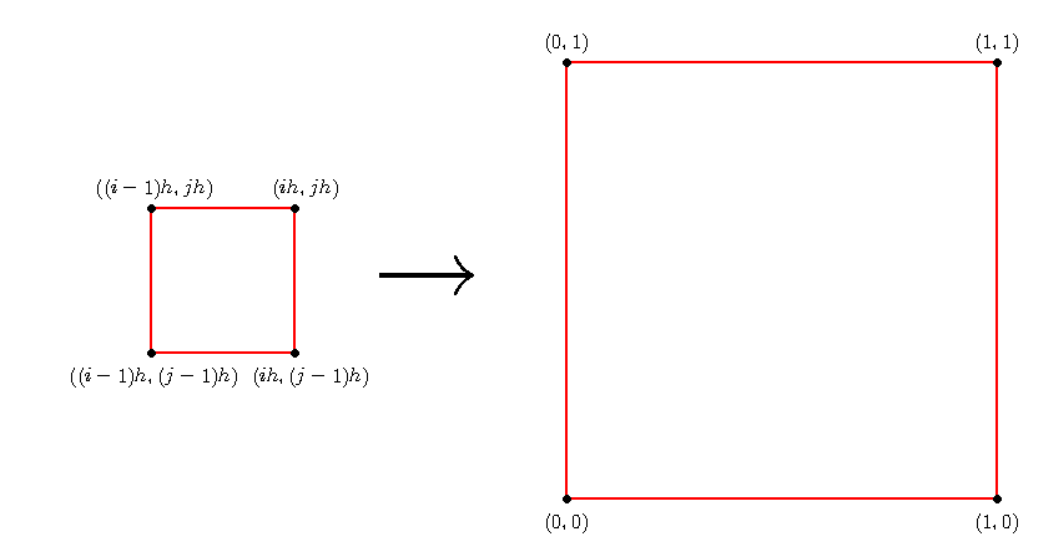
\includegraphics[width=10cm]{GridFigure/hCellTorefCell}
\caption{Figure to show conversion to reference cell}
\label{fig:refcell}
\end{figure}
Looking for the linear transformation that takes $x:[(i-1)h,ih] \rightarrow \hat x:[0,1]$ and $y:[(j-1)h,jh] \rightarrow \hat y:[0,1]$ we get that:
\begin{eqnarray*}
    x &=& h \hat x +(i-1)h,\\
    y &=& h \hat y +(i-1)h.
\end{eqnarray*}
Using the transformations we can now look at the locally defined stiffness ($\mathcal{K}_h$) and mass ($\mathcal{M}_h$) matrices:
$$ \mathcal{K}_h =  \int_{(i-1)h}^{ih}\int_{(j-1)h}^{jh} \curl \phiv_a \, \curl \phiv_b \, dx \, dy \, \mbox{ and } \, \mathcal{M}_h =   \int_{(i-1)h}^{ih}\int_{(j-1)h}^{jh} \phiv_a  \, {\cdot} \, \phiv_b\, dx \, dy$$

\subsubsection{Local Stiffness matrix}
Using the linear transformation with $\mathcal{K}_h$ we obtain
$$ \mathcal{K}_h =  \int_{(i-1)h}^{ih}\int_{(j-1)h}^{jh} \curl \phiv_a(\bar x,\bar y) \, \curl \phiv_b (\bar x,\bar y) \, dx \, dy $$
where $(\bar x, \bar y) = \big(\frac{x-(i-1)h}{h},\frac{y-(i-1)h}{h}\big)$. Hence we get the local stiffness matrix to be:
\begin{equation}
    \mathcal{K}_h = \begin{pmatrix}
        1&1&-1&-1\\1&1&-1&-1\\-1&-1&1&1\\-1&-1&1&1\\
    \end{pmatrix}
\end{equation}


\subsubsection{Local Mass matrix}

Now, using the linear transformations as we used to compute $\mathcal{K}_h$, then the local Mass matrix is
\begin{equation}
    \mathcal{M}_h = \frac {h^2}{6} \begin{pmatrix}
         2 & 0 & 1 & 0\\ 0 & 2 & 0 & 1\\ 1 & 0 & 2 & 0\\ 0 & 1 & 0 & 2\\
    \end{pmatrix}
\end{equation}

\subsubsection{Local Load vector}
For the load vector (the right-hand-vector) the usual thing to do is to use some sort of quadrature to approxomate the following integral:
$$  \mathpzc{f}_h =\int_{(i-1)h}^{ih}\int_{(j-1)h}^{jh} \f (x,y) \, \cdot \, \phiv_b  \bigg(\frac{x-(i-1)h}{h},\frac{y-(i-1)h}{h}\bigg)\, dx. $$
Generally one would use a first or second order approximation (midpoint rule or 2-point Gaussian quadrature) for this integral as we are using linear basis functions in the FEM scheme.
% Using the basis function in (\ref{eq:BasisFuncsQuads}), the local stiffness and mass matrices

\subsection{Assembling linear system}

Once the local stiffness and mass matrices as well as the local load vector are compute then it is time to assemble the global system $$\mathcal{A} u = \mathpzc{f}.$$
where $\mathcal{A} = \mathcal{K}+\mathcal{M}$. This is a fairly simple process in which we loop though all the elements and add in the contributions form the stiffness and mass matrices into there correct place in the global matrix $\mathcal{A}$  (see the pseudo-code below).

\noindent\fbox{%
\begin{varwidth}{\dimexpr\linewidth-2\fboxsep-2\fboxrule\relax}
\begin{algorithmic}
\For {k =1:NumCells}

$el$=NNode(k,:)
   \For {i =1:4}
      \For {j =1:4}

       \hspace{10mm}    $\mathcal{A}(el$(i),$el$(j)) =  $\mathcal{A}(el$(i),$el$(j)) +$\mathcal{K}_h$(i,j) + $\mathcal{M}_h$(i,j)

       \EndFor

    $\mathpzc{f}(el$(i)) = $\mathpzc{f}(el$(i)) + $\mathpzc{f}_h$(i)

    \EndFor
\EndFor
\end{algorithmic}
\end{varwidth}
}

\subsection{Boundary Conditions}

So far we have not said anything about boundary conditions. In finite elements we have "essential boundary conditions" (conditions that we need to manually impose) and "natural boundary conditions" (conditions which are directly imposed by the variational form).



\section{MATLAB results}


\section{FEniCS results}


\subsection{Convergence results}

\begin{table}[H]
\begin{center}
\begin{tabular}{|l|c|c|c|c|}
\hline
cycle & \# cells & \# dofs & $L_2$-error\\
\hline
$0$ & $4$ & $56$ & $0.0575954$\\
            $1$ & $8$ & $208$ & $0.0292943$\\
            $2$ & $16$ & $800$ & $0.0147103$\\
            $3$ & $32$ & $3136$ & $0.00736305$\\
            $4$ & $64$ & $12416$ & $0.00368252$\\
            $5$ & $128$ & $49408$ & $0.00184138$\\
            $6$ & $256$ & $197120$ & $0.000920707$\\
            $7$ & $512$ & $787456$ & $0.000460355$\\

\hline
\end{tabular}
\end{center}
\end{table}

\begin{figure}[h!]
\centering
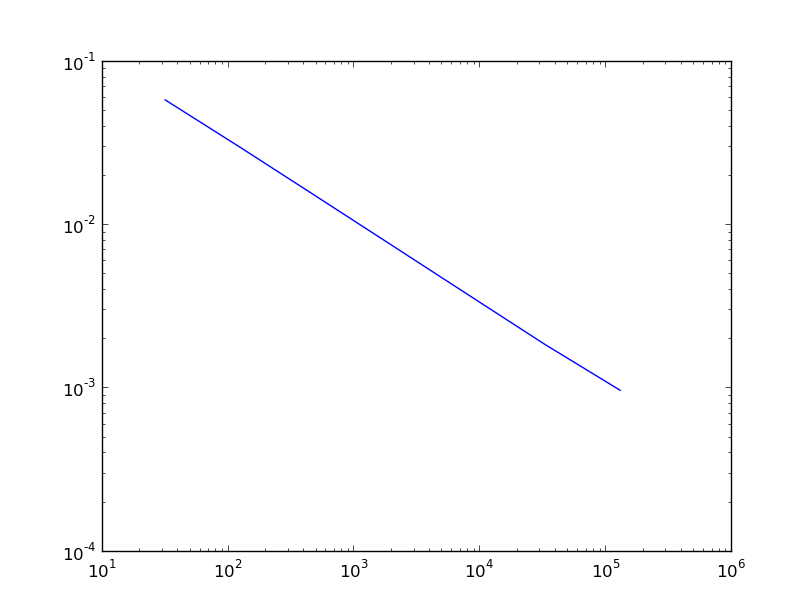
\includegraphics[width=15cm]{FEniCS_ConvergencePlot}
\end{figure}

\subsection{Matrix timing results}

\begin{table}[H]
\begin{center}
\begin{tabular}{|c|r|r|c|} \hline
cycle & \# cells & \# dofs & Time\\ \hline
$0$ & $4$ & $56$ & $0.022646$\\
            $1$ & $8$ & $208$ & $0.00144291$\\
            $2$ & $16$ & $800$ & $0.00212812$\\
            $3$ & $32$ & $3136$ & $0.00621486$\\
            $4$ & $64$ & $12416$ & $0.0200882$\\
            $5$ & $128$ & $49408$ & $0.079313$\\
            $6$ & $256$ & $197120$ & $0.366703$\\
            $7$ & $512$ & $787456$ & $1.55944$\\
            $8$ & $1024$ & $3.14778e{+06}$ & $6.79219$\\
            $9$ & $2048$ & $1.2587e{+07}$ & $27.8257$\\

\hline
\end{tabular}
\end{center}
\end{table}
\begin{figure}[h!]
\centering
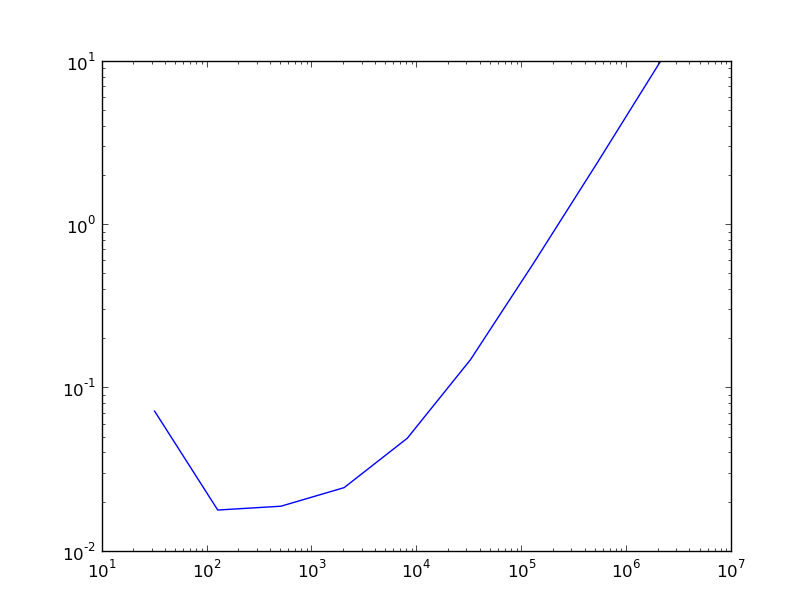
\includegraphics[width=15cm]{FEniCS_timing}
\end{figure}




 \subsection{None zero boundary conditions}
%

\section{deal.II results}

\subsection{Convergence results}

\begin{table}[H]
\begin{center}
\begin{tabular}{|c|r|r|c|} \hline
cycle & \# cells & \# dofs & $L_2$-error\\
0 & 16 & 40 & 3.3545e-01\\
1 & 64 & 144 & 1.6312e-01\\
2 & 256 & 544 & 8.0546e-02\\
3 & 1024 & 2112 & 4.0129e-02\\
4 & 4096 & 8320 & 2.0046e-02\\
5 & 16384 & 33024 & 1.0021e-02\\
6 & 65536 & 131584 & 5.0101e-03\\
\hline
\end{tabular}
\end{center}
\end{table}



\begin{figure}[h!]
\centering
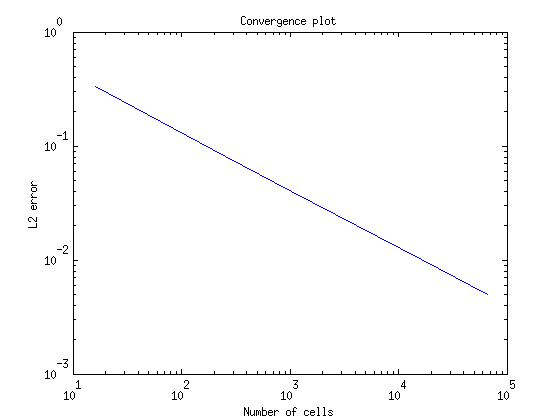
\includegraphics[width=15cm]{ConvergencePlot}
\end{figure}

\subsection{Matrix timing results}

\begin{table}[H]
\begin{center}
\begin{tabular}{|c|r|r|c|} \hline
cycle & \# cells & \# dofs & Time\\
0 & 16 & 40 & 0.0016\\
1 & 64 & 144 & 0.0045\\
2 & 256 & 544 & 0.0173\\
3 & 1024 & 2112 & 0.0662\\
4 & 4096 & 8320 & 0.2582\\
5 & 16384 & 33024 & 1.0823\\
6 & 65536 & 131584 & 4.1593\\
7 & 262144 & 525312 & 16.8618\\
8 & 1048576 & 2099200 & 67.1105\\ \hline
\end{tabular}
\end{center}
\end{table}


\begin{figure}[h!]
\centering
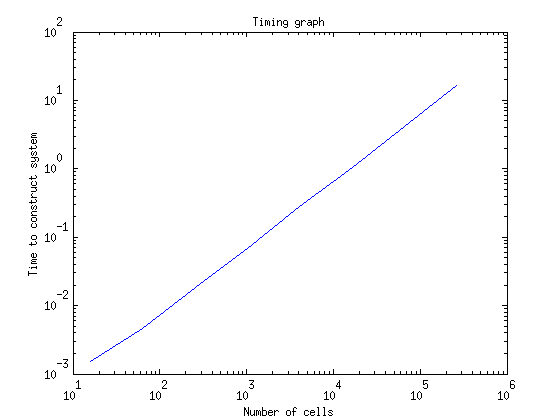
\includegraphics[width=15cm]{TimingsPlot}
\end{figure}
 \subsection{None zero boundary conditions}
%
% \cite{Schneebeli2003}







\bibliographystyle{apalike}
\bibliography{../../../../References/MHD,../../../../References/Electromagnetics,../../../../References/Fluids,../../../../References/FEM}


\end{document}
